\subsubsection{Generalizing Contract Access Control}

In order to generalize \solt{contract} access control we introduce:

\begin{enumerate}
  \item \sol{interface Authority}, which defines \solt{function}[s] to
    determine whether some \emph{subject} is permitted to access some
    \emph{resource},
  \item \sol{contract Authorization}, which defines a \solt{modifier} for
    restricting access to \solt{function} calls based on an \solt{address}, and
  \item \sol{contract Guard}, a convenience \solt{contract}, which provides an
    implementation of \sol{interface Authorization} by aggregating
    implementations of \sol{interface Authority}.
\end{enumerate}

These components combined allow us to provide a generalized access control
model; separating the responsibilities of Authorization, deferring
Authorization.\footnotemark{}
\todo{Alternative names: Guard, Authority, Enforcer, Authorization}

\footnotetext{
  I think I would maybe prefer \sol{interface Authorization} to define
  \sol{isAuthorized} and for \sol{interface Authority} to define
  \sol{getAuthority} and \sol{setAuthority}.

  A better name in that case might be \sol{interface AuthorityManager}.
}

\begin{figure}[H]
    \centering
    \caption{Generalized contract access control.}% \label{fig:authorization}
    \figurepdf[]{guard}
    % 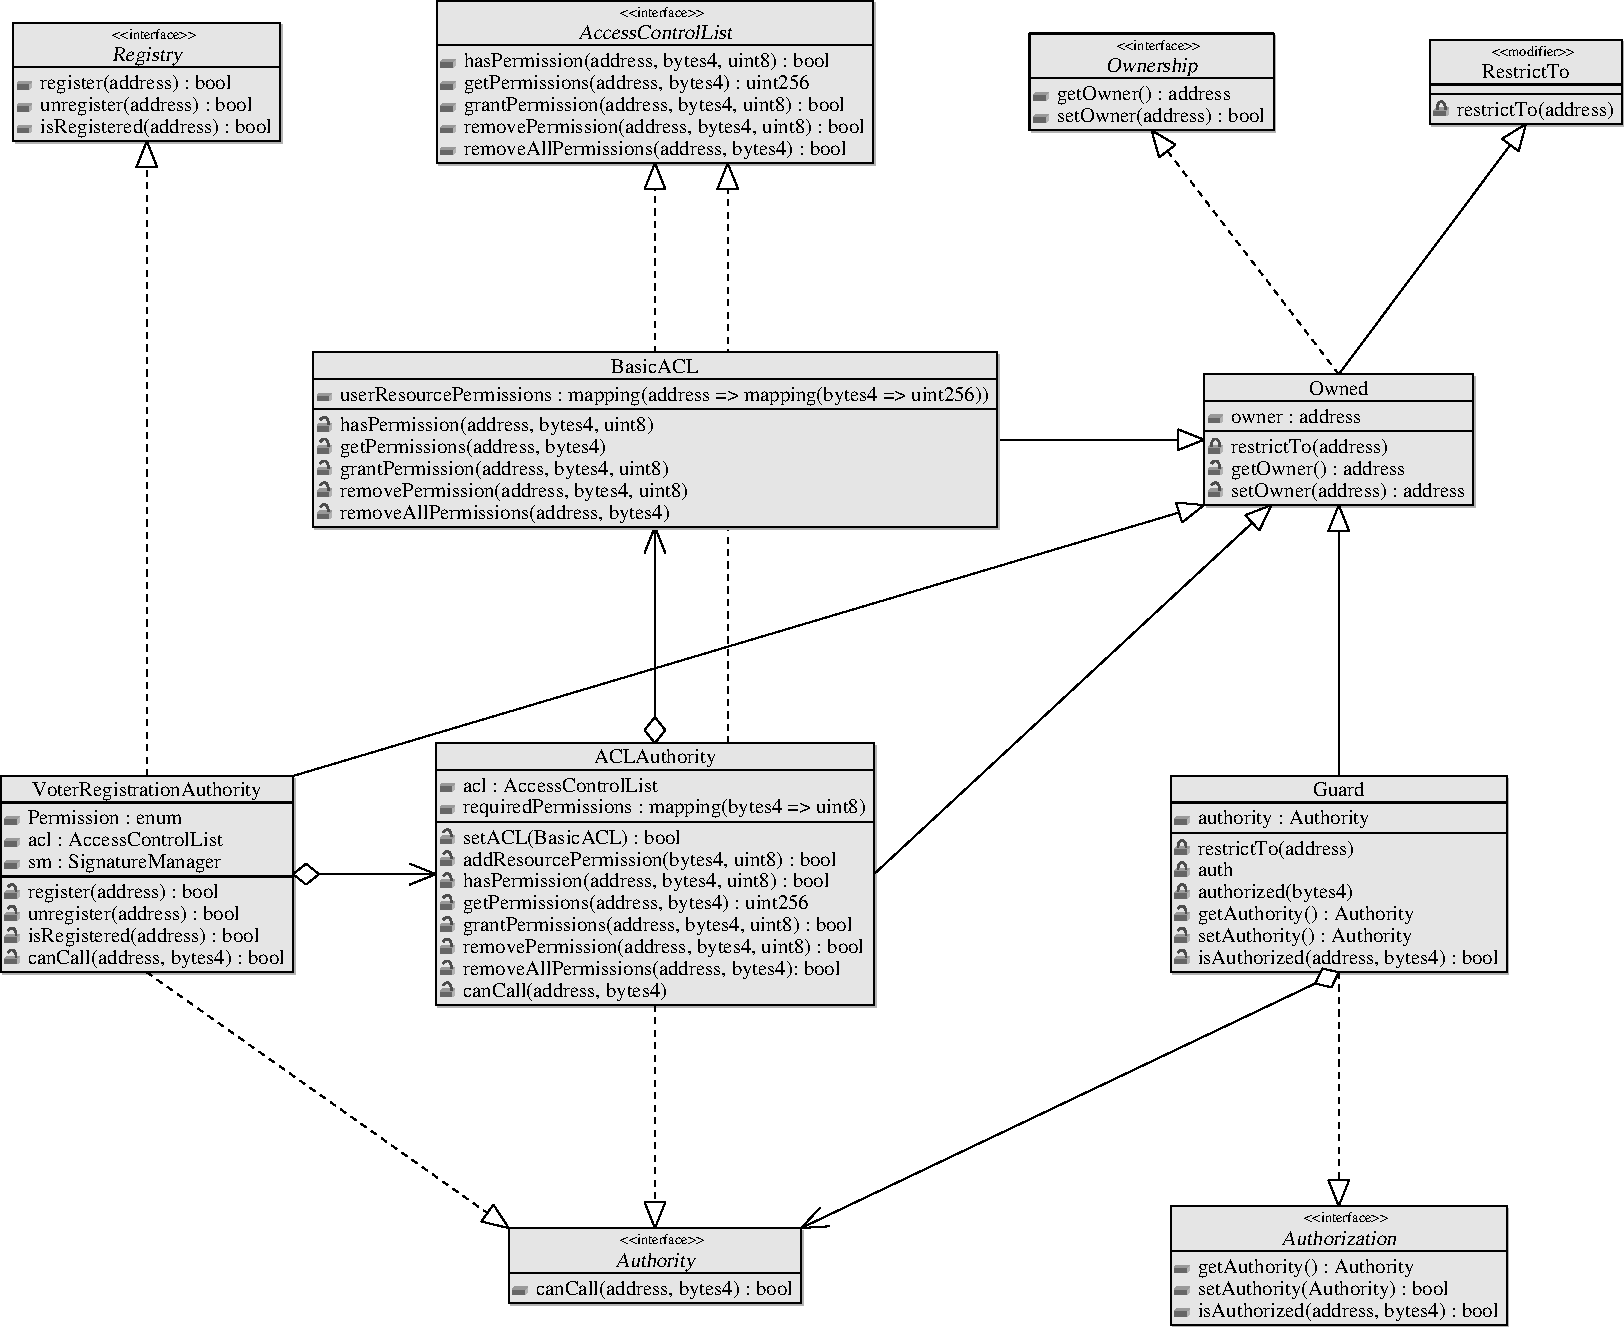
\includegraphics[width=\textwidth]{figures/authorization/figure}
    % \includestandalone[width=\textwidth]{\fig{authorization}}
\end{figure}

\subsubsection{Interface Authority}

The \solt{interface}, \sol{interface Authority}, introduces functionality for
managing whether some \emph{subject}, typically an Ethereum account represented
by \solt{address}, can access some \emph{resource}, typically an Ethereum
\solt{function} represented by \solt{function} signature, \solt{bytes4}. By
defining the \emph{resource} by it's \solt{function} signature and not by a
specific \solt{function} owned by a specific \solt{contract} we leave open the
possibility for managing \solt{contract} access control across
\solt{contract}[s], a functionality which will be necessary to build
pseudo-centralized registration authorities.

\begin{solidity}[interface Authority]
interface Authority {
  function canCall (address _subject, bytes4 _resource) public constant returns (bool _canCall);
}
\end{solidity}

\begin{interface}
  \begin{functions}
    \item \sol{function canCall (address _subject, bytes4 _resource)}, evaluates
      whether some \emph{resource}, \solt{contract function}, can be used by
      some \emph{subject}, Ethereum account.

      \begin{parameters}
        \item \sol{address _subject}, the \emph{subject}, Ethereum account,
          whose permissions are being evaluated.\footnotemark{}

          \footnotetext{
            The \solt{address} of the \emph{subject} may be \emph{any} Ethereum
            account, including \emph{contract accounts}.
          }

        \item \sol{bytes4 _resource}, the \emph{resource}, \solt{contract
          function}, which the \emph{subject's} permissions are being evaluated
          against.
      \end{parameters}

      \begin{returns}
        \item \sol{bool _canCall}, resolves to \solt{true} if the
          \emph{subject}, \sol{address _subject}, is permitted to access the
          \emph{resource}, \sol{bytes4 _resource}, otherwise \solt{false}.
      \end{returns}
  \end{functions}
\end{interface}


\subsubsection{Interface Authorization}

The \solt{interface}, \sol{interface Authorization}, introduces functionality
for managing authorities, \sol{function getAuthority()} and \sol{function
setAuthority()}, and also functionality similar to that of an \solt{Authority},
\sol{function isAuthorized()}.% \footnotemark{}

% \footnotetext{
%   If I don't update this to just be \sol{interface AuthorityManager} then I
%   should \emph{really} update \sol{interface Authority} to supply
%   \sol{function isAuthorized ()}, instead of \sol{function canCall()}, and
%   update this \solt{interface} to implement/extend \sol{interface Authority}.
% }

\begin{solidity}[interface Authorization]
interface Authorization {
  function getAuthority () public constant returns (address _authority);
  function setAuthority (address _authority) public returns (bool _success);
  function isAuthorized (address _subject, bytes4 _resource) public returns (bool _isAuthorized);
}
\end{solidity}

\begin{interface}
  \begin{functions}
    \item \sol{function getAuthority ()}, returns the \solt{address} of a
      \solt{contract} which implements the \solt{interface Authority}.

      \begin{returns}
        \item \sol{address _authority}, the \solt{address} of a \solt{contract}
          which implments the \solt{interface Authority}.
      \end{returns}

    \item \sol{function setAuthority (address _authority)}, updates the state of
      the \solt{contract} to to reflect the new \solt{contract} which provides
      an implementation of the \solt{Authority interface}.
      \todo{
        Make sure the Guard checks that the contract actually implements the
        interface!!!
      }

      \begin{parameters}
        \item \sol{address _authority}, the \solt{address} of a \solt{contract}
          which implements the \solt{interface Authority}.
      \end{parameters}

      \begin{returns}
        \item \sol{bool _success}, resolves to \solt{true} if the operation was
          successful; otherwise \solt{false}.
      \end{returns}

    \item \sol{function isAuthorized (address _subject, bytes4 _resource)},
      evaluates whether some \emph{subject}, Ethereum account, is authorized to
      access some \emph{resource}, \solt{contract function}.

      \begin{parameters}
        \item \sol{address _subject}, the \emph{subject}, Ethereum account,
          whose permissions are being evaluated.\footnotemark{}

          \footnotetext{
            The \solt{address} of the \emph{subject} may be \emph{any} Ethereum
            account, including \emph{contract accounts}.
          }

        \item \sol{bytes4 _resource}, the \emph{resource}, \solt{contract
          function}, which the \emph{subject's} permissions are being evaluated
          against.
      \end{parameters}

      \begin{returns}
        \item \sol{bool _isAuthorized}, resolves to \solt{true} if the
          \emph{subject}, \sol{address _subject}, is permitted to access the
          \emph{resource}, \sol{bytes4 _resource}, otherwise \solt{false}.
      \end{returns}
  \end{functions}
\end{interface}


\subsubsection{Contract Guarded}

The \solt{contract}, \sol{contract Guarded}, is a \solt{contract} which offers a
convenient mechanism for easily integrating generalized \solt{contract} access
control functionality; e.g., \sol{contract MyContract is Guarded {}}.
\solt{contract Guarded}, by virtue of implementing the \solt{Authorization
interface}, supports deferring access control responsibilities to an external
\solt{contract} which implements the \solt{Authority interface} while leaving
open the possibility for a \solt{contract} to provide its own access control
implementation by itself implementing the \solt{Authority interface}.

\todo{If I'm changing this from Guard to Guarded then I need to update all of
the references to Guard.}

\begin{solidity}[contract Guarded]
contract Guarded is Owned, Authorization {
  Authority public authority;

  function getAuthority () public constant returns (address _authority) {
    return address(authority);
  }

  function setAuthority (address _authority) public auth returns (bool _success) {
    authority = Authority(_authority);
    return true;
  }

  function isAuthorized (address _subject, bytes4 _resource) public returns (bool _isAuthorized) {
    if (_subject == address(this)) return true;
    if (authority == Authority(0)) return false;
    if (_subject == owner) return true;
    return authority.canCall(_subject, _resource);
  }

  modifier auth {
    assert(isAuthorized(msg.sender, msg.sig));
    _;
  }

  modifier authorized (bytes4 _resource) {
    assert(isAuthorized(msg.sender, _resource));
    _;
  }
}
\end{solidity}

\begin{code}
  \begin{modifiers}
    \item \sol{modifier auth ()}, restricts access to \solt{function} calls
      based on an \solt{address} provided.

      \begin{displayquote}
        Restriction to \solt{function}[s] is accomplished by comparing the
        \solt{address} of the \solt{function} \emph{caller}, \sol{msg.sender},
        against the configured \solt{address}, \sol{address _subject}. If the
        \solt{address} of the \solt{msg.sender} does not match the
        \solt{address} of the \solt{_subject} then the \solt{require} statement
        will force the immediately arrest of \solt{contract} evaluation,
        \solt{revert} the \emph{state} of the \solt{contract}, refund any
        remaining \solt{gas}, \solt{gasleft()}, to the \emph{caller}, and
        exit.\footnotemark{}

        \todo{Should notes be documented differently?}
      \end{displayquote}

      \footnotetext{
        Note that the \emph{caller}, \sol{msg.sender}, of the \solt{function}
        will not necessarily be an \emph{external account}, e.g., human user;
        the \emph{caller} of the \solt{contract} \solt{function} may itself also
        be a \solt{contract}, i.e., a \emph{contract account}, which is calling
        the \solt{contract} \solt{function} from its own \solt{contract}
        \solt{function}.
      }

      \begin{parameters}
      \item \sol{address _subject}, the \emph{subject} who is to be granted
        access to the \solt{function}.

        \begin{displayquote}
          The \solt{address} of the \emph{subject} may be \emph{any} Ethereum
          account, including \emph{contract accounts}.
        \end{displayquote}
      \end{parameters}

    \item \sol{modifier authorized (address _resource)}, restricts access to
      \solt{function} calls based on an \solt{address} provided.

      \begin{displayquote}
        Restriction to \solt{function}[s] is accomplished by comparing the
        \solt{address} of the \solt{function} \emph{caller}, \sol{msg.sender},
        against the configured \solt{address}, \sol{address _subject}. If the
        \solt{address} of the \solt{msg.sender} does not match the
        \solt{address} of the \solt{_subject} then the \solt{require} statement
        will force the immediately arrest of \solt{contract} evaluation,
        \solt{revert} the \emph{state} of the \solt{contract}, refund any
        remaining \solt{gas}, \solt{gasleft()}, to the \emph{caller}, and
        exit.\footnotemark{}

        \todo{Should notes be documented differently?}
      \end{displayquote}

      \footnotetext{
        Note that the \emph{caller}, \sol{msg.sender}, of the \solt{function}
        will not necessarily be an \emph{external account}, e.g., human user;
        the \emph{caller} of the \solt{contract} \solt{function} may itself also
        be a \solt{contract}, i.e., a \emph{contract account}, which is calling
        the \solt{contract} \solt{function} from its own \solt{contract}
        \solt{function}.
      }

      \begin{parameters}
      \item \sol{address _subject}, the \emph{subject} who is to be granted
        access to the \solt{function}.

        \begin{displayquote}
          The \solt{address} of the \emph{subject} may be \emph{any} Ethereum
          account, including \emph{contract accounts}.
        \end{displayquote}
      \end{parameters}
  \end{modifiers}
\end{code}

